\section{Practical Methodology}
\begin{multicols}{2}
	\subsection{Performance Metrics}
	\begin{align*}
	\text{Precision} &= \frac{t_p}{t_p+f_p} & \text{Recall} &= \frac{t_p}{t_p+f_n}\\
	\text{Specificity} &= \frac{t_n}{t_n+f_p} & \text{Accuracy} &= \frac{t_p+t_n}{t_p+t_n+f_p+f_n}\\
	\end{align*}
	\begin{itemize}
		\item Recall is also called \textbf{sensitivity}
		\item Specificity is also called \textbf{True negative rate}
	\end{itemize}
	Clearly there is a trade-off between precision and recall so a PR Curve is plotted to show this trade-off:
	\begin{figure}[H]
		\centering
		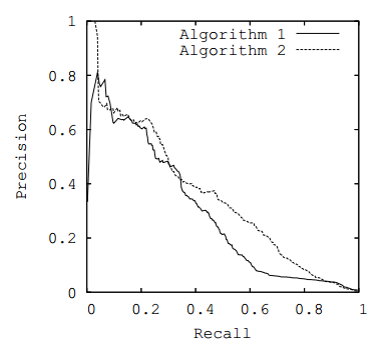
\includegraphics[width=0.75\linewidth]{images/pr_curve.png}
	\end{figure}
	If a curve is too much information, often the area under the curve is reported or alternatively the \textbf{F-score}:
	\[ F = \frac{2pr}{p+r} \]
	The fraction of examples for which the machine can make a confident decision is called the \textbf{coverage}.
	This is again a trade-off, the lower the coverage, the better the accuracy, since the machine only classifies the easy examples.\\

	To determine whether the training data is good enough, we can train the model until it's overfitted. The performance on the training set should be almost arbitrarily good.


	\subsection{Selecting Hyperparameters}
	Properly selected hyperparameters often make the difference between a well working scheme and a failed scheme.
	Basically one can find these hyperparameters by hand using experience or one can use an automated approach using experiments.
	This requires insight into the effect a hyperparameter has.
	The \textbf{table} shows some popular hyperparameters and their influence on the effective capacity.

	\subsection{Automatic Hyperparameter Optimization Algorithms}
	In principal, it should be possible to automatically find a good set of hyperparameters which results in an acceptable generalization error.
	These tuning schemes have their own new hyperparameters, but they tend to be less sensitive.\\

	\textbf{Grid Search: }If there are only a few parameters, a grid search is reasonable.
	For each hyperparameter a finite set of values needs to be defined, which should be explored.
	Then every possible combination of theses settings is evaluated and the setting resulting in the lowest test error is selected.

	\textbf{Random Search} is the preferred way of finding a good set of hyperparameters that converges much faster.
	The basic idea is, that for each hyperparameter a value is picked randomly.
	Now the test error for this random hyperparameter vector is calculated and the best vector is stored.

	\begin{figure}[H]
		\centering
		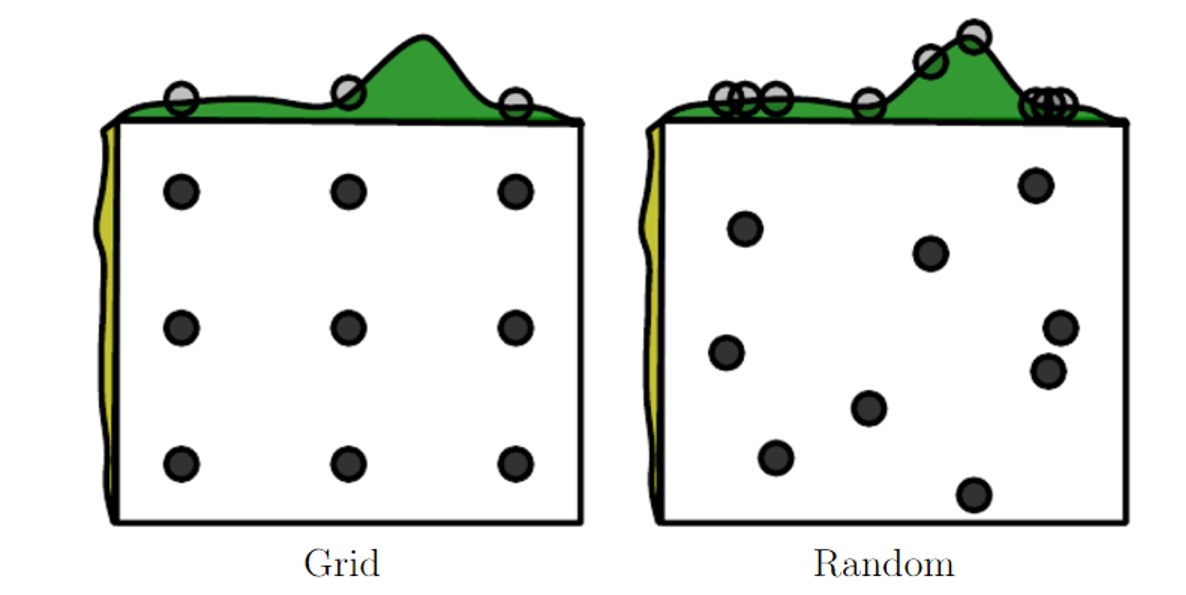
\includegraphics[width=0.75\linewidth]{images/gridrandom.PNG}
	\end{figure}

	\begin{figure}[H]
		\centering
		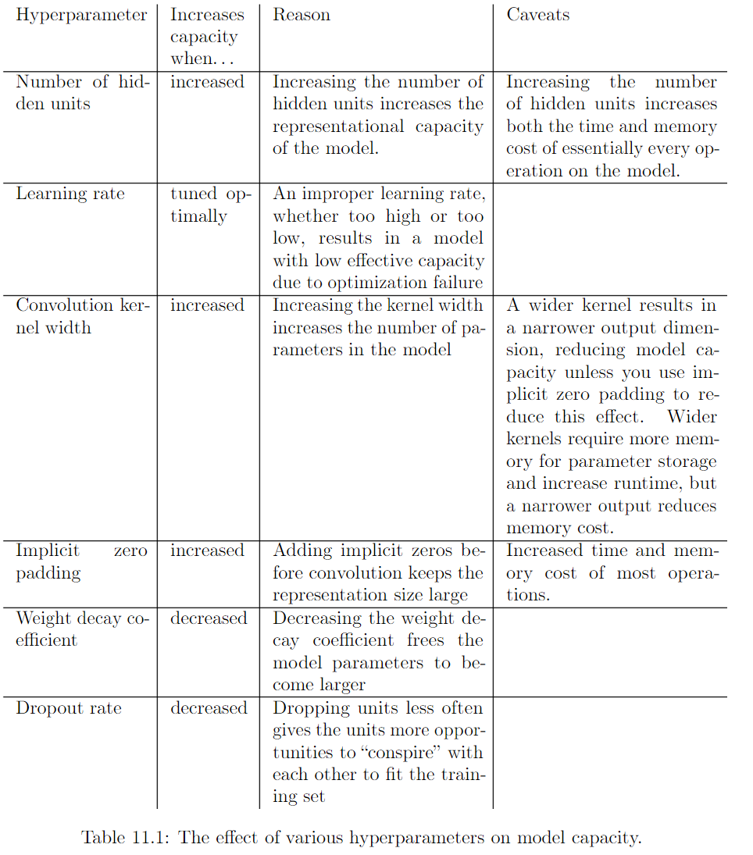
\includegraphics[width=1\linewidth]{images/hypertable.png}
	\end{figure}

\end{multicols}
